\chapter{Approach and Implementation}
\label{ch:approach}
%%%%%%%%%%%%%%%%%%%%%%%%%%%%%%%%%%%%%%%%%%%%%%%%%%%%%%%%%%%%%%%%%%%%%%%%%%%%%%%
%%%%%%%%%%%%%%%%%%%%%%%%%%%%%%%%%%%%%%%%%%%%%%%%%%%%%%%%%%%%%%%%%%%%%%%%%%%%%%%
%%%%%%%%%%%%%%%%%%%%%%%%%%%%%%%%%%%%%%%%%%%%%%%%%%%%%%%%%%%%%%%%%%%%%%%%%%%%%%%
%%%%%%%%%%%%%%%%%%%%%%%%%%%%%%%%%%%%%%%%%%%%%%%%%%%%%%%%%%%%%%%%%%%%%%%%%%%%%%%

This chapter describes the workflow and implementation I applied to reach my research goals.
The preparation and processing of the data are primarily driven by a combination of exploratory and iterative processes.

I primarily follow  Farine's and Whitehead's~\cite{farine2015constructing} steps and key considerations for social network analysis to non-human animal data.
[TODO: steps kurz zusammenfassen, und unterschiede zu mir erklären]
Figure~\ref{fig:process} visualizes the adapted and resulting process.
[TODO: Schritte im Bild nummerieren und im Text verwenden]

In the first step, the data set was analyzed to form a general understanding of the given dataset, its structure, quality, and characteristics.

The results of this investigation are used to define nodes and infer associations to build the network, respectively derive the parameters for the network pipeline.

The resulting networks are analyzed by using network science tools and methods.
[hier unbedingt methoden aufzählen]																																																																																																						

[TODO: umfomulieren, Begruendun Auswahl der Attribute, und welche Test habe ich genau gemacht.]
For testing underlying hypothesis the networks are attributed with the bees spatial information and their age.

\begin{figure}[htb]
	\centering
	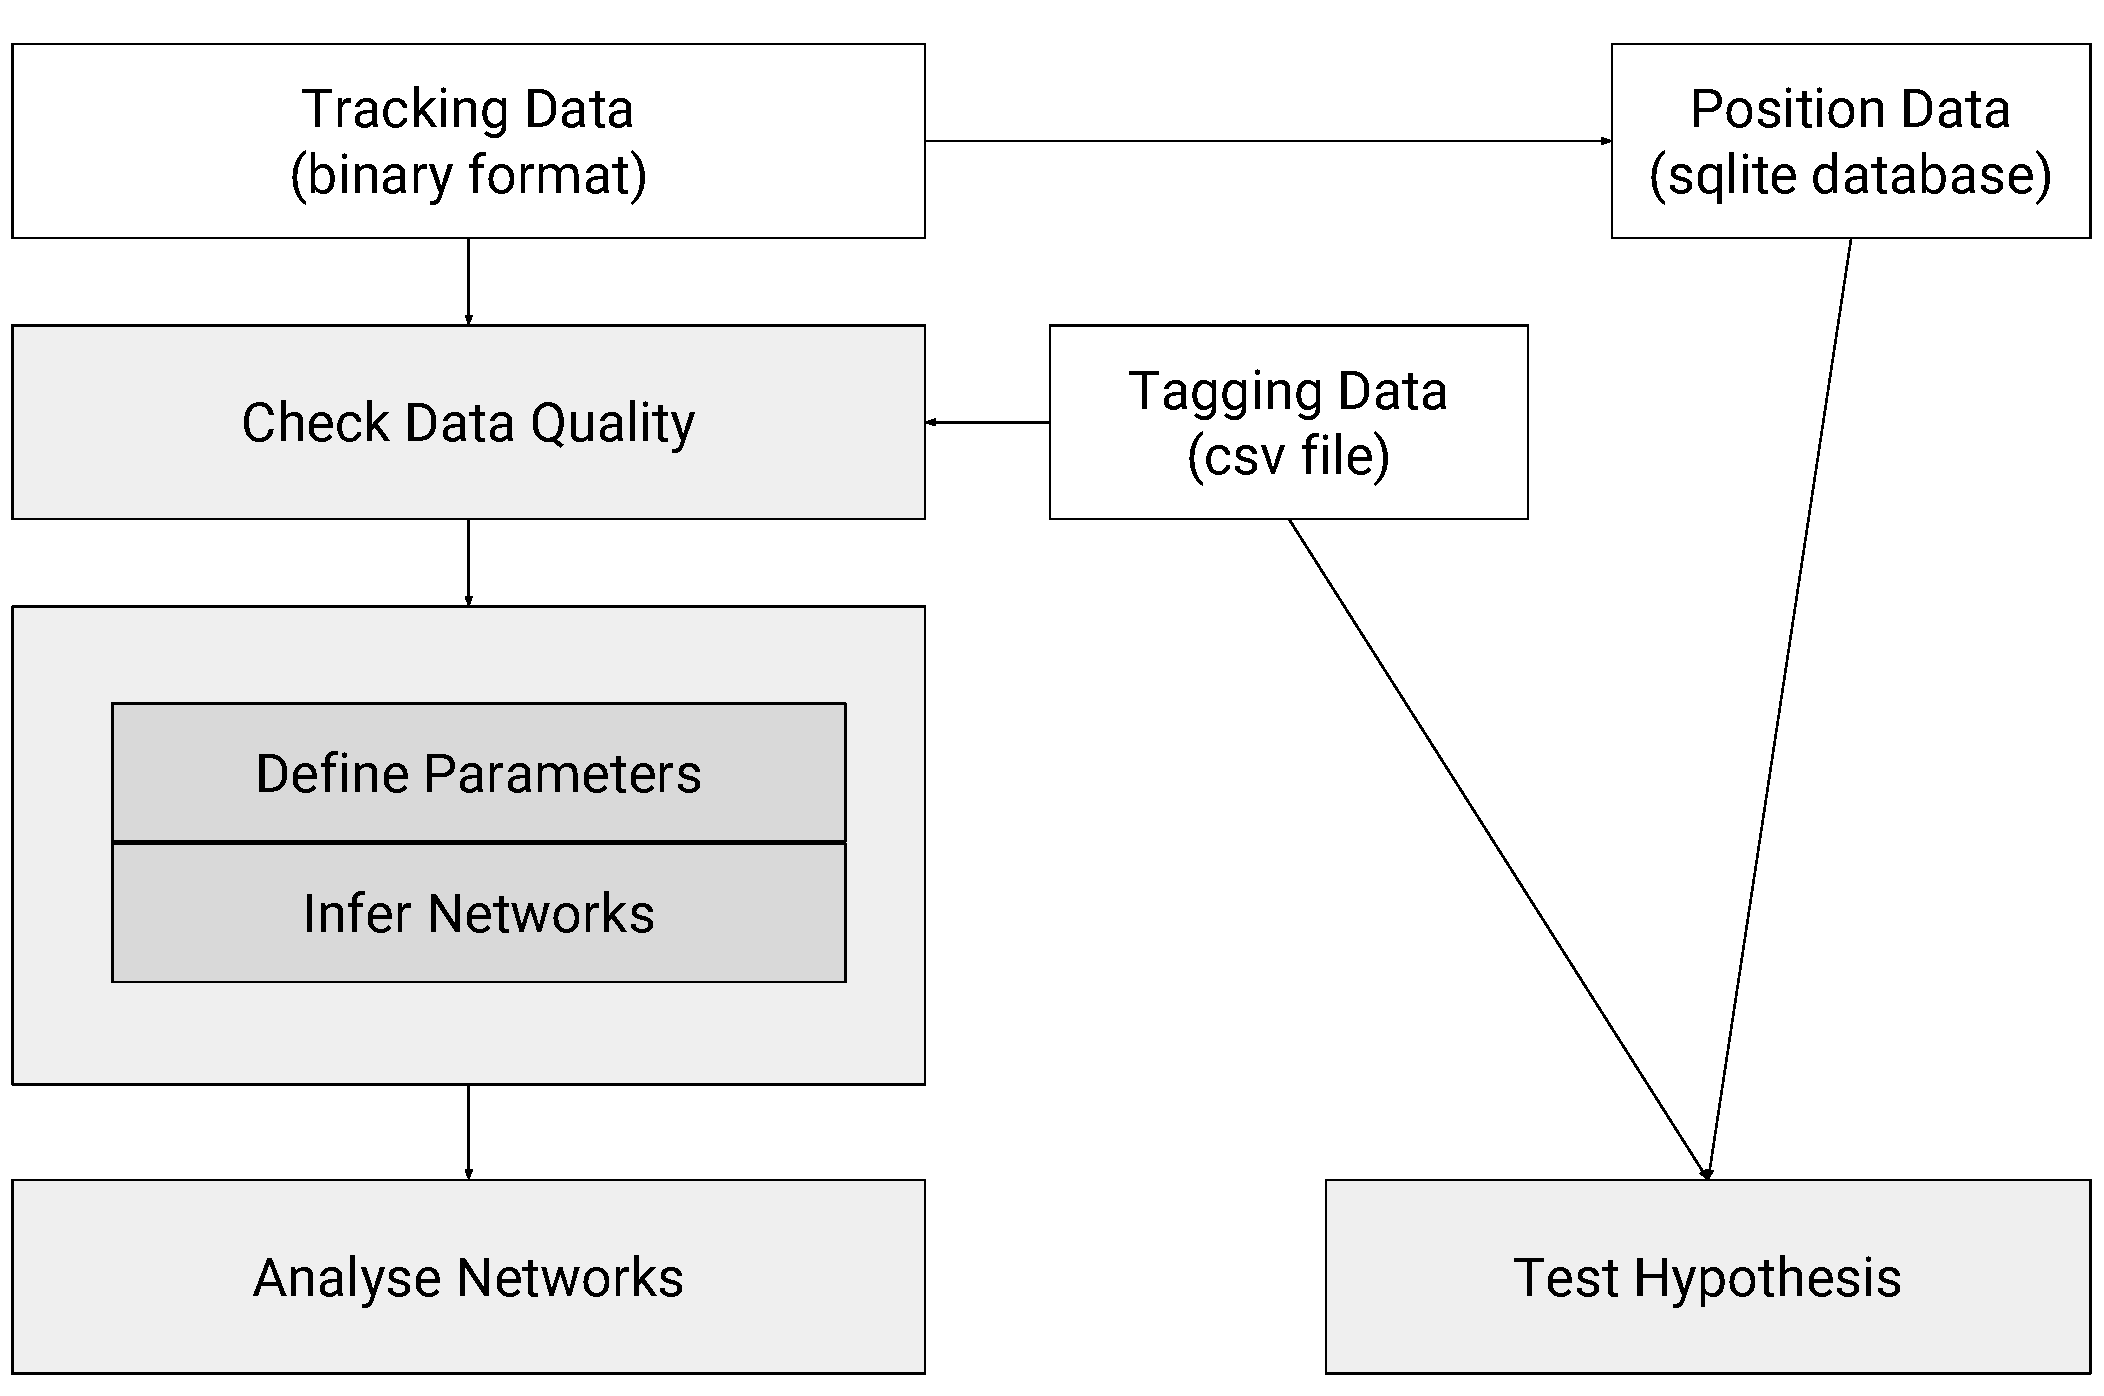
\includegraphics[width=0.8\textwidth]{Figures/process}
	\caption[Steps of the research approach]{\textbf{Steps of the research approach} [TODO: anpassen, iterationen, hypothesis raus, evtl. so viele Schritte im Bild wie Abschitte im Text, zumindest muss das irgendwie anders.]}
	\label{fig:process}
\end{figure}

%%%%%%%%%%%%%%%%%%%%%%%%%%%%%%%%%%%%%%%%%%%%%%%%%%%%%%%%%%%%%%%%%%%%%%%%%%%%%%%
%%%%%%%%%%%%%%%%%%%%%%%%%%%%%%%%%%%%%%%%%%%%%%%%%%%%%%%%%%%%%%%%%%%%%%%%%%%%%%%
%%%%%%%%%%%%%%%%%%%%%%%%%%%%%%%%%%%%%%%%%%%%%%%%%%%%%%%%%%%%%%%%%%%%%%%%%%%%%%%
%%%%%%%%%%%%%%%%%%%%%%%%%%%%%%%%%%%%%%%%%%%%%%%%%%%%%%%%%%%%%%%%%%%%%%%%%%%%%%%
\section{The Dataset}
\label{sec:dataset}
%%%%%%%%%%%%%%%%%%%%%%%%%%%%%%%%%%%%%%%%%%%%%%%%%%%%%%%%%%%%%%%%%%%%%%%%%%%%%%%
%%%%%%%%%%%%%%%%%%%%%%%%%%%%%%%%%%%%%%%%%%%%%%%%%%%%%%%%%%%%%%%%%%%%%%%%%%%%%%%
%%%%%%%%%%%%%%%%%%%%%%%%%%%%%%%%%%%%%%%%%%%%%%%%%%%%%%%%%%%%%%%%%%%%%%%%%%%%%%%
%%%%%%%%%%%%%%%%%%%%%%%%%%%%%%%%%%%%%%%%%%%%%%%%%%%%%%%%%%%%%%%%%%%%%%%%%%%%%%%

\begin{figure}
    \centering
    \begin{subfigure}[b]{\textwidth}
	\centering
	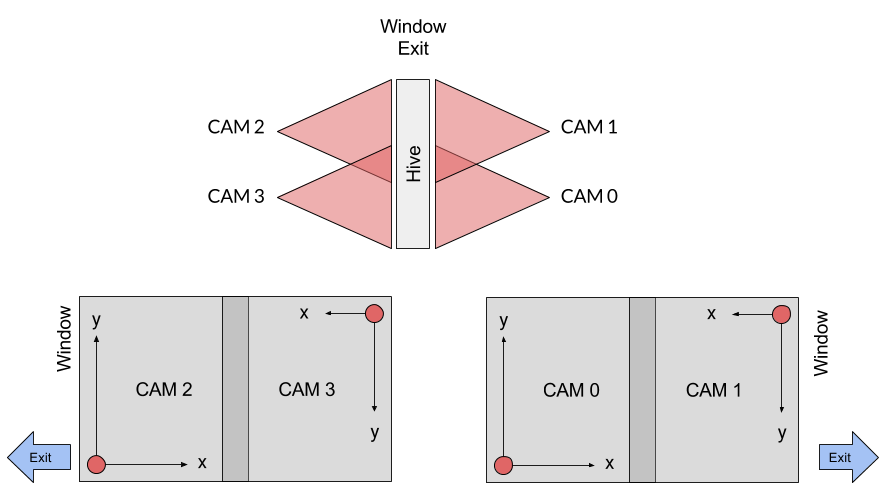
\includegraphics[width=0.8\textwidth]{Figures/setupCams}
	\caption[Camera setup]{\textbf{Camera setup} Each side of the honeycomb is filmed by two cameras. The two cameras per side overlap, bees inside this area are detected from both cameras.}
	\label{fig:cams}
	\vspace{5mm}
    \end{subfigure}
    \begin{subfigure}[b]{\textwidth}
	\centering
	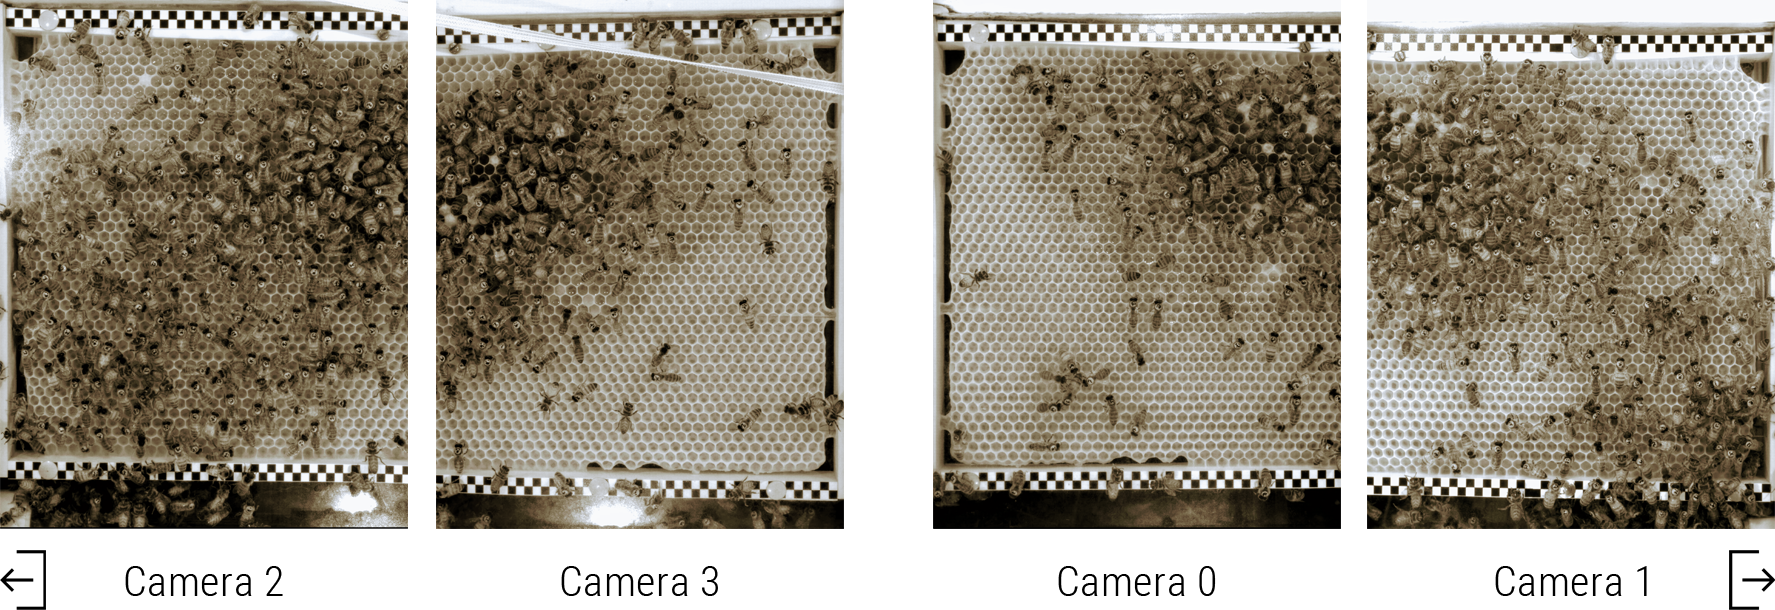
\includegraphics[width=0.65\textwidth]{Figures/beesClose}
	\vspace{5mm}
	\caption[Images for each camera]{\textbf{Images for each camera} Top: side~A, bottom: side~B}
	\label{fig:veryclose}
    \end{subfigure}
 	\caption[Observation setup]{\textbf{Observation setup}}
 	\label{fig:obssetup}
\end{figure}

The dataset derives from high resoluted video files, that capture tagged honey bees of one colony in an single-frame observation hive.
The colony includes about 3200 bees over a period of nine weeks. The bees are uniquely tagged with circular 12-bit markers (figure~\ref{fig:markers}, section~\ref{ch:intro}).
Two cameras per side filmed the complete honeycomb permanently.
Figure~\ref{fig:cams} illustrates the camera setup.
The \emph{recording period} lasted nine weeks (63 days), from 19.07.2016 until 19.09.2016, with some interruptions due to maintenance work and technical failures. An overview about the complete reocrding period is given in figure~\ref{fig:observation-period} in appendix~\ref{ch:appendix}.

All four cameras, each with a resolution of $4000\times3000$ pixels, record $3.5$ frames per second. 
An image analysis pipeline~\cite{wario2015automatic} detects all bees in each frame.
The resulting detection data is stored in a binary file format.
An python library\footnote{The library is called \texttt{bb-binary} and is created by the Biorobotics Lab. It can be found on GitHub: \url{https://github.com/BioroboticsLab/bb_binary}; Last accessed: 2106-02-16, 04:28PM} provides an frame-level access to those binary files.
The size of the dataset is $470$~GB, about $7.5$~GB of binary data per day.

The 67 days long \emph{tagging period} started on 28.06.2016 and lasted until 02.09.2016, resulting in $3.191$ tagged bees. The young bees, which were raised in a separate incubator, were tagged and then added to the observation hive, about noon each day. Figure~\ref{fig:tagging-period} (Appendix~\ref{ch:appendix}) shows the frequency of tagged bees per day. The hatching day for each bee is documented; therefore the age of each bee at a particular point in time can be calculated.

[TODO: Begruendung des gewaehlten Zeitraumes: Funktionstüchtigkeit und Altersverteilung]
For further analysis, I chose three days: 20., 22., and 24. August.

\clearpage
%%%%%%%%%%%%%%%%%%%%%%%%%%%%%%%%%%%%%%%%%%%%%%%%%%%%%%%%%%%%%%%%%%%%%%%%%%%%%%%
%%%%%%%%%%%%%%%%%%%%%%%%%%%%%%%%%%%%%%%%%%%%%%%%%%%%%%%%%%%%%%%%%%%%%%%%%%%%%%%
\subsection{Data Scheme}
\label{subsec:datascheme}
%%%%%%%%%%%%%%%%%%%%%%%%%%%%%%%%%%%%%%%%%%%%%%%%%%%%%%%%%%%%%%%%%%%%%%%%%%%%%%%
%%%%%%%%%%%%%%%%%%%%%%%%%%%%%%%%%%%%%%%%%%%%%%%%%%%%%%%%%%%%%%%%%%%%%%%%%%%%%%%

\begin{table}[!t]
\colorbox{usethiscolorhere}{
\centering
\begin{tabularx}{\textwidth}{@{} r Y @{}}
	\textbf{Frame container} &
	A container for all frames, which belong to a specific video file of a certain camera.\\
	\textbf{Frame} &
	This includes all detections of one camera image at a certain point in time.\\
	\textbf{Detection} &
	A detection of a bee at a certain point in time.\\
	\textbf{Decoded ID} &
	Identifier of a bee consisting of 12 probability values, representing 12 bits.\\
	\textbf{Confidence} &
	Value between 0\% and 100\%.\\
	\textbf{ID} &
	The decimal representation of an decoded ID, after applying a certain confidence value.\\
	\textbf{Bee time series} & Binary sequence, indicating the absence and presence of a certain bee in a particular time interval.\\
	\textbf{Pair time series} & Binary sequence, indicating the absence and presence of two bees in a particular time interval.\\
\end{tabularx}
}
\end{table}

The data is organized in so-called \emph{frame containers}.
Each frame container corresponds to one video file of a single camera and consists of about $1024$ \emph{frames}. So the frame container specifies the camera (\emph{camId}), which recorded the video.
Each frame holds a list of bees, which were detected by the image analysis pipeline and is attributed with a \emph{timestamp}.

A bee \emph{detection} has, among others, the following attributes:

\begin{table}[!h]
\centering
\begin{tabular}{rl}
\textbf{xpos}: & $x$ coordinate of bee with respect to the image in pixel \\
\textbf{ypos}: & $y$ coordinate of bee with respect to the image in pixel \\
\textbf{decoded ID}: & decoded 12-bit ID \\
\textbf{cam ID}: & ID of the camera ${0,1,2,3}$ \\
\textbf{timestamp}: & unix timestamp with milliseconds\\
\end{tabular}
\end{table}

The data can be accessed by iterating on the frame level, using a start and end time\-stamp for specifying a time interval. The complete data scheme can be found on GitHub\footnote{\url{https://github.com/BioroboticsLab/bb_binary/blob/master/bb_binary/bb_binary_schema.capnp}; Last accessed: 2106-02-16, 04:46PM}. 



%%%%%%%%%%%%%%%%%%%%%%%%%%%%%%%%%%%%%%%%%%%%%%%%%%%%%%%%%%%%%%%%%%%%%%%%%%%%%%%
%%%%%%%%%%%%%%%%%%%%%%%%%%%%%%%%%%%%%%%%%%%%%%%%%%%%%%%%%%%%%%%%%%%%%%%%%%%%%%%
\subsection{ID Probabilities, Confidence Level, and Quality}
\label{subsec:confidence}
%%%%%%%%%%%%%%%%%%%%%%%%%%%%%%%%%%%%%%%%%%%%%%%%%%%%%%%%%%%%%%%%%%%%%%%%%%%%%%%
%%%%%%%%%%%%%%%%%%%%%%%%%%%%%%%%%%%%%%%%%%%%%%%%%%%%%%%%%%%%%%%%%%%%%%%%%%%%%%%

\begin{figure}
    \centering
    \begin{subfigure}[b]{0.45\textwidth}
        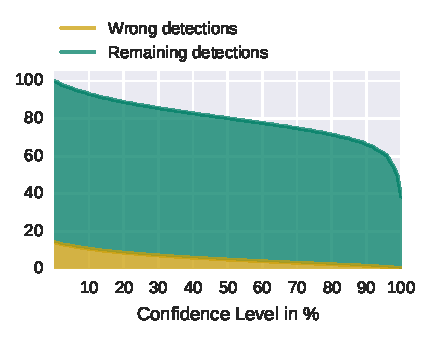
\includegraphics[width=\textwidth]{Figures/detectionsWrongConf}
        \caption[Detections]{\textbf{Detections}}
        \label{fig:detections}
    \end{subfigure}
    \begin{subfigure}[b]{0.45\textwidth}
        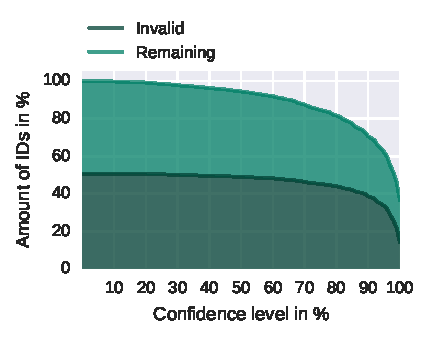
\includegraphics[width=\textwidth]{Figures/idsWrongConf}
        \caption[IDs]{\textbf{IDs}}
        \label{fig:ids}
    \end{subfigure}
 	\caption[Quality of detections and IDs]{\textbf{Quality of detections and IDs} \emph{Green} represents the number of remaining detections and remaining IDs (from $4096$ possible IDs). \emph{Yellow} indicates the fraction of wrong IDs and wrong detections in relation the remaining number of IDs and detections.\protect\footnotemark}
 	\label{fig:remainingVSquality}
\end{figure}

\footnotetext{Data set: 26.07.2016, 4~p.~m., 10~minutes, all cameras}

Twelve bits can encode the identity of 4096 bees.
Each bit of the decoded ID is not a one or zero but represents a probability between $0$ and $255$, normalized to a value between $0$ and $1$.
Therefore, a bit indicates the confidence of the image analysis pipeline for that specific bit.
I define the confidence $c$ for a bit $b$, analogously to Leon~\textcite[p.~14]{leon2016}, as $c(b)=2\cdot|b-0.5|$.
The confidence of a decoded ID is, accordingly, the minimum of all twelve bits' confidences.
Consequently, a high level of confidence reduces the amount of data, which remains for further processing.

I use the age information of the bees to check the quality of the remaining data.
The age is specified in days.
An age of $0$ days indicates that a bee was born on that day.
It is possible that the resulting age is below $0$ days.
One the one hand, this happens when the pipeline detected a bee, that was not born yet.
On the contrary, this can happen, if it discovered a bee tag, that was never used during the study, then the age is set to $-100$ days.

I examined (1) the number of detections and (2) the number of unique IDs, depending on the chosen confidence.

For (1) I calculated the age of each bee detection.
A detection with a negative age is counted as a \emph{wrong detection}.
I assumed that a similar number of wrong detections also occurred among detections with a positive age, but remained unseen; therefore I doubled the error\footnote{I chose the 26.07.2016 for testing this because half of the bee tags ($2014$ out of $4096$) were already assigned.}.
For (2), analogously a unique ID with a negative age is counted as a \emph{wrong ID}. The total amount of wrong IDs is doubled.

As expected, with increasing confidence, the number of remaining detections and the amount of remaining unique IDs decreased (figure~\ref{fig:remainingVSquality}).
Also even though the number of wrong detections decreases steadily with an increasing confidence level, the number of wrong IDs only starts to decline with a very high level of confidence.
With a confidence level of 100\%, 30.2\% of the remaining unique IDs are invalid, corresponding to only 2.5\% of invalid detections.

Therefore, to obtain a more reliable dataset, invalid detections need to be filtered out, independently of the confidence value.
The amount of data that remains for further processing is still highly dependent on the chosen level of confidence.

%%%%%%%%%%%%%%%%%%%%%%%%%%%%%%%%%%%%%%%%%%%%%%%%%%%%%%%%%%%%%%%%%%%%%%%%%%%%%%%
%%%%%%%%%%%%%%%%%%%%%%%%%%%%%%%%%%%%%%%%%%%%%%%%%%%%%%%%%%%%%%%%%%%%%%%%%%%%%%%
\subsection{Time Series of Bees and Bee Pairs}
\label{subsec:tracking}
%%%%%%%%%%%%%%%%%%%%%%%%%%%%%%%%%%%%%%%%%%%%%%%%%%%%%%%%%%%%%%%%%%%%%%%%%%%%%%%
%%%%%%%%%%%%%%%%%%%%%%%%%%%%%%%%%%%%%%%%%%%%%%%%%%%%%%%%%%%%%%%%%%%%%%%%%%%%%%%

The dataset, is transformed to binary \emph{bee time series}, depicted in figure~\ref{fig:structure} (left and middle). A time series of a bee is a sequence of zeros and ones indicating the absence and presence of a bee over a specified time interval. 
I examined the effect the level of confidence has on the bee time series.
As expected, with an increasing confidence level the average gap length decreases and the overall number of gaps increases (figure~\ref{fig:gaps}).

The number of gaps, those bee time series has, is important because in a later step I want to extract pairs of close bees, who are present at the very same time. I call those \emph{pair time series}, as shown in figure~\ref{fig:structure} (right). So a lot of gaps in bee time series could lead to a lot of gaps in the pair time series.

\begin{figure}[htb]
	\centering
	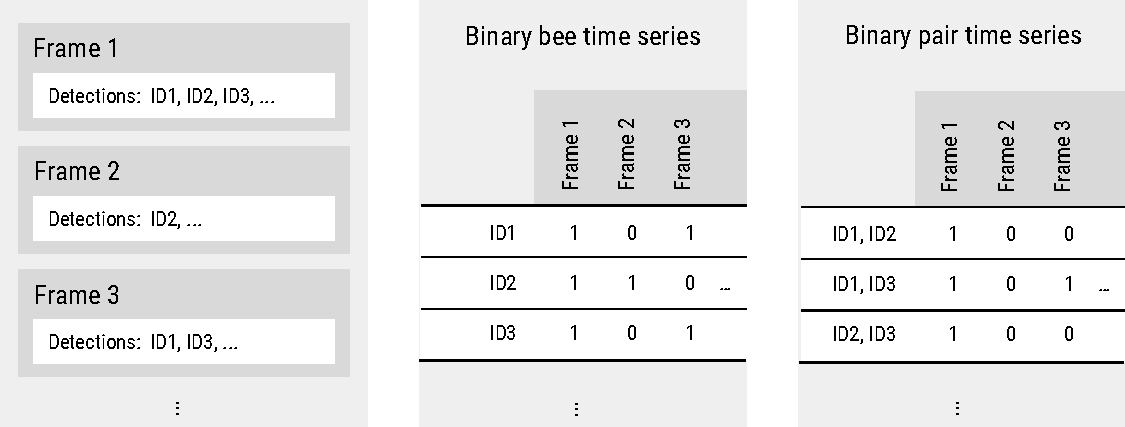
\includegraphics[width=1.0\textwidth]{Figures/structure}
	\caption[Structure of dataset]{\textbf{Structure of dataset} \emph{Left}: original dataset - containing a sequence of frames with bee detections; \emph{Middle:} binary bee time series - zero and one indicate absence and presence of a bee; \emph{Right:} binary pairs time series - zero and one indicate the absence and presence of two bees in the same frame.}
	\label{fig:structure}
\end{figure}

\begin{figure}[htb]
	\centering
	\begin{subfigure}[b]{0.45\textwidth}
		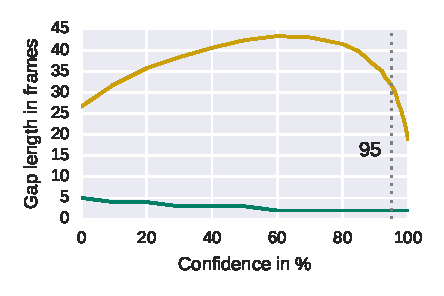
\includegraphics[width=\textwidth]{Figures/gaplen}
		\caption[Length of gaps]{\textbf{Length of gaps}}
		\label{fig:gaplen}
	\end{subfigure}
	\begin{subfigure}[b]{0.45\textwidth}
		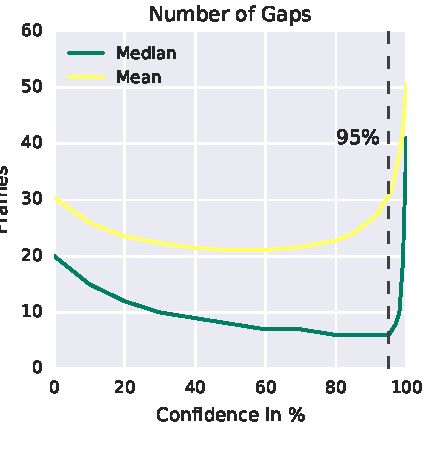
\includegraphics[width=\textwidth]{Figures/numgaps}
		\caption[Number of gaps]{\textbf{Number of gaps}}
		\label{fig:numgaps}
	\end{subfigure}
	\caption[Influence of Confidence Level on Gaps]{\textbf{Influence of confidence level on gaps} [TODO: add legend][TODO:gaps D] With an increasing level of confidence the average gap length decreases and the number of gaps per bee series increases. \emph{Orange} indicates the median, \emph{green the mean}.\protect\footnotemark }
	\label{fig:gaps}
\end{figure}

\footnotetext{Data set: 26.07.2016, 16:00-16:05}


%%%%%%%%%%%%%%%%%%%%%%%%%%%%%%%%%%%%%%%%%%%%%%%%%%%%%%%%%%%%%%%%%%%%%%%%%%%%%%%
%%%%%%%%%%%%%%%%%%%%%%%%%%%%%%%%%%%%%%%%%%%%%%%%%%%%%%%%%%%%%%%%%%%%%%%%%%%%%%%
\subsection{Detection Frequency Filter}
%%%%%%%%%%%%%%%%%%%%%%%%%%%%%%%%%%%%%%%%%%%%%%%%%%%%%%%%%%%%%%%%%%%%%%%%%%%%%%%
%%%%%%%%%%%%%%%%%%%%%%%%%%%%%%%%%%%%%%%%%%%%%%%%%%%%%%%%%%%%%%%%%%%%%%%%%%%%%%%
A good indicator, whether a bee is alive and present on a particular day, is its detection frequency. The hypothesis is: Bees who have a low detection rate are not physically present in the hive, respectively do not exists at that day.
To check this hypothesis, I investigate whether there is a correlation between the age of bees and their detection frequency.

\begin{figure}[t]
	\centering
	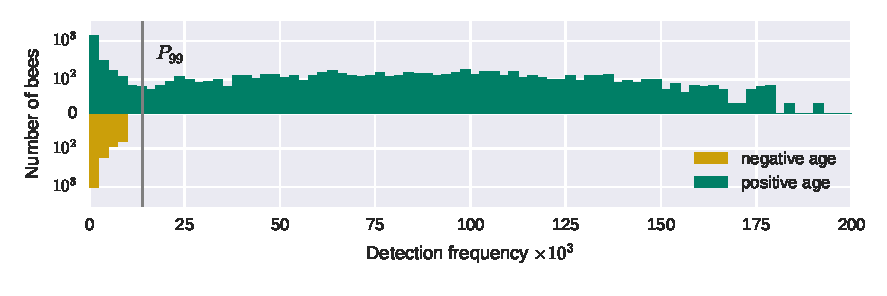
\includegraphics[width=1.0\textwidth]{Figures/filter}
	\caption[Detection frequency of IDs]{\textbf{Detection frequency of IDs} [TODO: add legend] \emph{Orange} coressponds to bees with a negative age and \emph{green} displays bees with a positive age.\protect\footnotemark}
	\label{fig:filter}
\end{figure}

\footnotetext{Data set: 20.08.2016, 24 hours, number of total frames: 302400}

Bess with a negative age are on average detected less frequently than bees with a positive age.
In advance, I excluded bees from the statistics, which had a negative age, but a detection frequency over 10000 frames. Their detection frequency is similar to that from bees with a positive age. I looked at the corresponding photos taken by the camera and confirmed that those are living bees and no artifacts.\footnote{Probably a mistake in the table, which reports the hatching days for each bee.}
Also I excluded bees~($n=10$), whose age is unknown\footnote{id= [2,
    74,
    2045,
    3172,
    3764,
    3796,
    3827,
    3836,
    3844,
    3940]}.

For each analysis day, the number of detections per ID is obtained, excluding the mentioned IDs.
Additionally, I discarded all detections with an ID frequency below the 99th percentile of negative IDs.
A list of valid IDs per day is kept to filter out wrong detections beforehand.

%%%%%%%%%%%%%%%%%%%%%%%%%%%%%%%%%%%%%%%%%%%%%%%%%%%%%%%%%%%%%%%%%%%%%%%%%%%%%%%
%%%%%%%%%%%%%%%%%%%%%%%%%%%%%%%%%%%%%%%%%%%%%%%%%%%%%%%%%%%%%%%%%%%%%%%%%%%%%%%
\subsection{Implications}
%%%%%%%%%%%%%%%%%%%%%%%%%%%%%%%%%%%%%%%%%%%%%%%%%%%%%%%%%%%%%%%%%%%%%%%%%%%%%%%
%%%%%%%%%%%%%%%%%%%%%%%%%%%%%%%%%%%%%%%%%%%%%%%%%%%%%%%%%%%%%%%%%%%%%%%%%%%%%%%
The confidence level is set to 95\%.
This a good balance between gaps in the time series and quality of the data and amount of remaining data.
Because bee time series contain a lot of short gaps (mean = 3, 95\% confidence), the inference of edges (bees that are spatially close to each other at the same time), should take this into account.

\clearpage
\section{Inferring Networks}

The following part describes the pipeline for generating spatial proximity networks out of honey bee tracking data. A node in the network is a bee. They are distinguished by IDs. Only bees are in the network who interact at least once with another bee.

undirected and weighted, aggregated networks\\

Two bees are associated (spatially close to each other), if their distance is minor to a \emph{maximum distance}. As everything is very close in a bee hive this value is hard to choose. Only this criteria is very week, meaning having a resolution of three frames per seconds results in interactions which could only last for $0.33$ seconds. So an additional parameter the \emph{minimum contact duration} is introduced, it is the minimum time they have to spend at least nearby to be called associated.

Taking the fragmentation of tracks into account, it is obvious that two bees could be nearby but not at the very same time, but slightly shifted. So the minimum contact duration would be too errow prone. To overcome this issue one could correct the bee tracks, by filling gaps of varius sizes and interpolating the position of that bee accordingly. This is rather time consuming for this amount of tracking data (TODO: naja so doll auch nicht) and also considering, that the tracking data is going to be improved in the future, then manipulating the raw data seems senseless. I rather perform a gap filling (maybe similar to binary dilation?) on the time series of pairs, but not on the bee tracks, because this is independent of the input data.

Edges are attributed with two parameters. The first one is the frequency of contacts, so how often they share a close position. The second parameter is the total duration of contact, how many time frames in total they spend close by.

\subsection{Network Pipeline}

The network pipeline takes as input a path to the bb-binary data and outputs a graph in graphML file format. The pipeline takes the following parameters:

\begin{itemize}
\item path to data
\item confidence in percent
\item gap size in frames - this is used to corret the time series of bee pairs
\item maximum distance in px - define what close means (spatial proximity)
\item minimum contact duration in frames - how many frames bees need to spend nearby
\item cutoff in percent - IDs with a number of total detections below X percent of the mean frequency are discarded 
\item start timestamp - start of network slice
\item window size in minutes - size of time window for aggregating the network
\item number of used CPUs for parallelization
\item year - calculate IDs and set camera setup for 2015 or 2016
\end{itemize}

The pipeline is parallelized on frame level, that means, each process gets a portion (frames for a timeinterval of five minutes) of the data and extracts interactions/edges. The main process adds everything up and creates a network.
The steps are the following:

\begin{enumerate}
\item \textbf{Filter detections by confidence}\\
For each of the four camera the detections are filtered by the confidence level.

\item \textbf{Simple stitching}\\
Each side of the hive consists of two cameras. 	The $x$-coordinates of each detection (of the right	cameras) is moved further to the right, also adding an offset of $2\times \texttt{maximum distance}$. So the left and the right detection of each side of the hive are move into one reference system.

\item \textbf{Syncronize Cameras}\\
For each side of the hive the cameras need to be syncronized. In the normal case the difference between consecutive frames should be about $0.332$~seconds, due to technical problem this value can be lower ($0.003$ ) and higher ($2.932$) at certain times. Cameras 3 and 2 and cameras 1 and 0 are matched, frames without a match are dropped (shorter number of frames, matchen, threshold $0.33/2$, minimum).

\item \textbf{Discard Detections with certain IDs}\\
All detections whos ID is in a list are keept, other detections are discarded. (see frequency filter)

\item \textbf{Extract close pairs}\\
For each side of the hive, all close pairs according to the maximum distance parameter are calculated and then joined together.

\item \textbf{Generate time series of bee pairs}\\
The data structure (frames and detection) is transformed to time series of bee pairs.

\item \textbf{Correct pair time series.}\\
The time series of bees are corrected by filling in the gaps of length \texttt{gap size}.

\item \textbf{Extract edges}\\
The edges and its attributes (frequency and duration) are extracted from the time series of bees using the minimum contact duration parameter. A sequence of at least X ones counts as one interaction. The frequency of those series adn the total duration (number of ones) are the attributes.


\end{enumerate}

\subsection{Pipeline Parameters}
For performing the network analysis, I chose the pipeline parameters as follows:

\begin{description}
\item[Confidence] As explained in section\ref{subsec:confidence}, the confidence is set to $95\%$.

\item[Maximum Distance] I chose the length of a bee body, according to \textcite{baracchi2014socio}, as the maximum distance between two bees (figure~\ref{fig:radius}). The average bee length of $212$px ($\pm 16$px)  was determinded by manually measuring the length of all bees ($n=337$) in four images (one for each camera, 21.07.2016, 03:00PM) using the tool ImageJ\footnote{\url{http://imagej.net/Welcome}; Last accessed: 22.02.2016}.

\item[Gap Size] The gap size is set to two frames. This value corresponds to the median gap length in the time series of pairs ($\texttt{mode}=1$, $\texttt{mean}=27$). [TODO: what dataset was used (95\% confidence, XXX\% cutOff, XXXpx maximal distance, date, camera)]

\item[Minimum Contact Duration] This is set to three frames (one second). This corresponds to~\textcite{mersch2013tracking}, they as well exclude interactions below one second. Looking at the frequency distribution of chains of ones ($1$, $11$, $111$, and so on) of the pair time series (after filling the gaps), then: $\texttt{mode}=1$, $\texttt{median}=2$ and $\texttt{mean}=4$. Three frames corresponds to $57\%$ of all chains, this seem to be reasonable. [TODO: what dataset was used (95\% confidence, XXX\% cutOff, XXXpx maximal distance, date, camera)]

\end{description}

\begin{figure}[htb]
	\centering
	\begin{subfigure}[b]{0.4\textwidth}
		\centering
		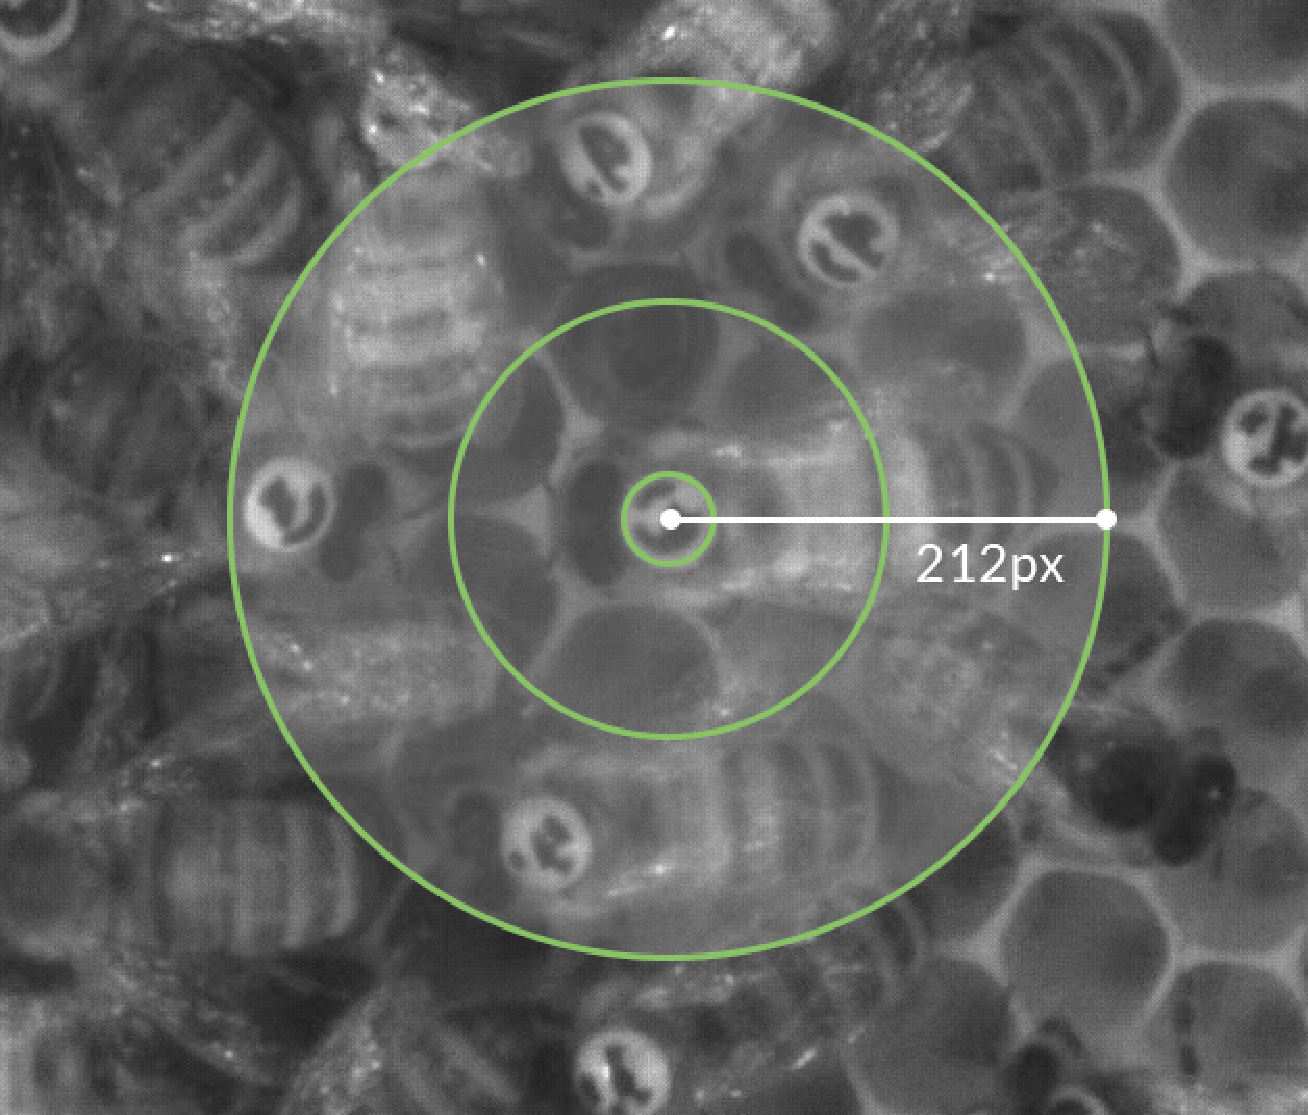
\includegraphics[width=\textwidth]{Figures/radius}
		\caption[Contact Radius]{Contact Radius}
		\label{fig:radius}
	\end{subfigure}
	\begin{subfigure}[b]{0.4\textwidth}
		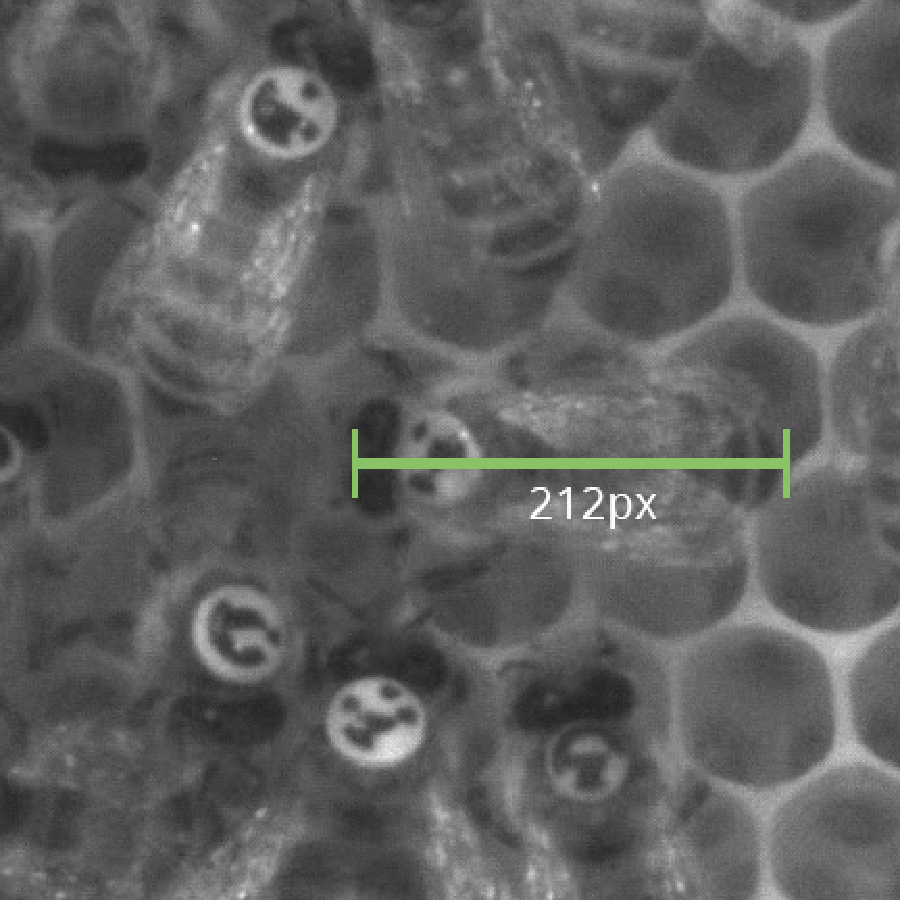
\includegraphics[width=\textwidth]{Figures/sizeTagBee}
		\caption[Bee and Tag Size]{Bee Length}
		\label{fig:size}
	\end{subfigure}
	\caption{Distance Between Bees: A length of a bee is chosen as the maximal  distance between bees.}
	\label{fig:contactRadius}
\end{figure}

\clearpage
\section{Static and Temporal Analysis}

Despite the possibility of generating networks of different granularity (resolution is minutes), here for further analysis daily networks (10h, two hours after sunrise until zwo hours before sunset) are aggregated.


\textcite{wey2008social}

\subsection{Static Network Analysis}
The following network properties were analysed for a static day and hour network.\\
TODO: list of properties. (similar to what others have done)
nodes, edges, density, diameter\\


\subsection{Temporal Analysis}
three day networks (2 days gap)\\
one network 2 weeks later\\

\subsection{Community Detection}
I tested all community detection algorithms implemented in python, to find an algorithm, which works well for my case of animal social networks. The three most common python libraries for network analysis were reviewed: NetworkX\footnote{\url{https://networkx.github.io/}; Last accessed: 16.03.2016, 6:36~p.m.}, igraph\footnote{\url{http://igraph.org/python/}; Last accessed: 16.03.2016, 6:38~p.m.}, and graph-tool\footnote{\url{https://graph-tool.skewed.de/}; Last accessed: 16:03.2016, 6:39~p.m.})

The algorithm needs to fulfill the following criteria:

\begin{itemize}
\item Support for large and very dense networks ($N>1000$, $D>50~\%$)
\item Support weighted edges
\item Fast runtime
\end{itemize}

Table~\ref{tab:algos} gives an overview about the twelve algorithms reviewed. Five algorithms did not terminate after 15~minutes and were therefore excluded from further investigations. Infomap and label propagation tend to partition all nodes into a single community, this is known especially in dense graphs~\cite{yang2016comparative, fortunato2010community}.
The Louvain algorithm is the same as multilevel, but takes longer producing almost the same communities and therefore was also excluded. Walktrap was tested for different step size parameters, as suggested in~\cite{pons2005computing}, the communities remained almost the same (only a few nodes switched communities). 

I had a closer look at fastgreedy, leading eigenvector, multilevel, and walktrap regarding the number of detected communities and community size for all three networks. Table~\ref{tab:algos4} shows the results. All algorithms found at least two communities. Except for leading eigenvector, there is a tendency that a third community exists.
I decided to use two algorithms for community detection: leading eigenvector and walktrap. \textcite{farine2015constructing} explains that leading eigenvector is often used with animal social networks and works well. Walktrap is chosen for also  examining the possible third community.

There are comparative analysis of community detection algorithms, e.g.~\cite{yang2016comparative, harenberg2014community}. They seem to be promising, but assume eighter a power law degree distribution or evaluate networks with a low density, which is not applicable here.

\begin{table}[htbp]
\small
\caption[Compairing community detection algorithms]{\textbf{Comparing community detection algorithms} Comparison of algorithms implemented in python. Criterias are the support of weighted edges, runtime and number of communities. A runtime indicated by $-$ mean no termination after 15~minutes.\\
}
\label{tab:algos}

\begin{tabularx}{\textwidth}{lcccccccccccc}
\toprule
	 {} &
	 \rotatebox{90}{\textbf{fastgreedy$^1$}} &
	 \rotatebox{90}{\textbf{leading eigenvector$^1$}} &
	 \rotatebox{90}{louvain$^2$} &
	 \rotatebox{90}{\textbf{multilevel$^1$}} &
	 \rotatebox{90}{\textbf{walktrap$^1$}} &
	 
	 \rotatebox{90}{infomap$^1$} &
	 \rotatebox{90}{label propagation$^1$} &
	 
	 \rotatebox{90}{edge betweenness$^1$} &
	 \rotatebox{90}{k-clique communities$^2$\thinspace} &
	 \rotatebox{90}{optimal modularity$^1$} &
	 \rotatebox{90}{spinglass$^1$} &
	 \rotatebox{90}{statistical inference$^3$} \\ \midrule
	 
	 
	 
	 Edge weights & $\times$ & $\times$ & $\times$ & $\times$ & $\times$ & $\times$ & $\times$ & & $\times$ & $\times$ & $\times$ \\ \midrule
	 Runtime in sec & ~$3.6$ & ~$6.3$ & $11.7$ & ~$0.7$ & $19.4$ & $13.2$ & ~$0.2$ & $-$ & $-$ & $-$ & $-$ & $-$ \\ \midrule
	 Communities & $3$ & $2$ & $2$ & $3$ & $2$ & $1$ & $1$ & $-$ & $-$ & $-$ & $-$ & $-$ \\ \midrule
	  & 473 & 488 & 469 & 462 & 490 & 922 &  922 &  &  &  &  &  \\
	  & 434 & 434 & 453 & 427 & 431 &  &  &  &  &  &  &  \\
	  & 15 &  &  & 33 & (1) &  &  &  &  &  &  &  \\
	 \bottomrule
	 
\end{tabularx}
\begin{flushright}
\footnotesize{
$^1$ igraph, $^2$ NetworkX, $^3$ graph-tool\\
}
\end{flushright}

\end{table}

% \hdashline
% \midrule
% \bottomrule
\begin{table}[htbp]
\centering
\caption[X]{\textbf{X} X\\
}
\label{tab:algos4}

\begin{tabular}{lcccc}
\toprule
	 {} &
	 fastgreedy &
	 leading eigenvector &
	 multilevel &
	 walktrap \\ \midrule
	 
	  Network 1
	  & 473 & 488 & 462 & 490 \\
	  & 434 & 434 & 427 & 431 \\
	  & 15 &   & 33 & (1) \\ \midrule
	  Network 2
	  & 504 & 503 & 481 & 372 \\
	  & 467 & 475 & 439 & 311 \\
	  & 7 &   &  58 & 294 \\
	  & & & & (1) \\ \midrule
	  Network 3
	  & 534 & 537 & 505 & 310 \\
	  & 388 & 385 & 415 & 390 \\
	  &  &   &  (2) & 231 \\
	 \bottomrule
	 
\end{tabular}

\end{table}

% \hdashline
% \midrule
% \bottomrule

\section{Attributed Data and Hypothesis Testing}
Hypothesis\\
(1) Communities reflect groups of bees working in different areas of the hive and\\
(2) Communities reflect different age groups\\

The data which was used to test the hypothesis (1) is saved in a sqlite database for faster access, because using bb\_binary (parsing the data over and over again) was to slow. For testing if lists of positions (spatial ditribution) are different the test XY was used [TODO: what to use here]

For hypothesis (2) the data is stored as a csv file of birth dates of each bee. For testing if age goups are different the Kolmogorov Smirnov Test was used.
\section{Implementation, Runtime and Complexity}
For implementing the network pipeline python, with pandas and numpy, are used, because the bb\_binary library, for accessing the tracking, data is only available in python. The networks, in graphML format, are created using the python library \emph{NetworkX}\footnote{\url{https://networkx.github.io/} ; Last accessed: 2017-02-17, 08:07PM} in version 1.11.
I used iGraph for community detection. Some bash scrips for generating multiple networks.

Bottleneck is reading bb\_binary data into pandas dataframes.
i used the multithreading for distributing the data an alevel of 5 minutes (a process the frames coresponding to 5 minutes).

Maybe some table with how long what step needs, with how many cores (hom much RAM and so on).